Minecraft � um jogo virtual que pode auxiliar no desenvolvimento de conhecimentos relacionados a espa�o e forma. � poss�vel criar casas, edif�cios, monumentos e at� naves espaciais, tudo em escala real, atrav�s do empilhamento de cubinhos. 
Um jogador deseja construir um cubo com dimens�es 4 x 4 x 4. Ele j� empilhou alguns dos cubinhos necess�rios. conforme a figura. 

\begin{figure}[h]
\centering
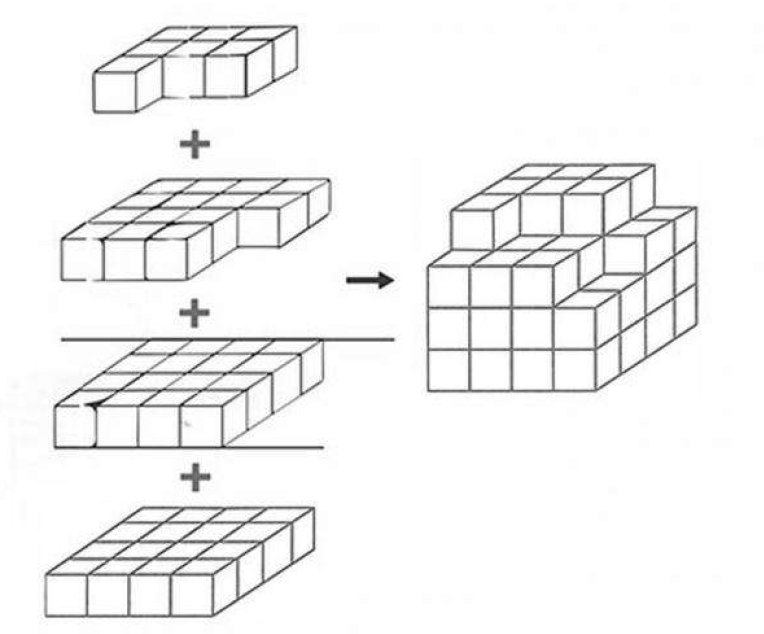
\includegraphics[width=8cm]{../figuras/q169(1)-2018}
\end{figure}

Os cubinhos que ainda faltam empilhar para finalizar a constru��o do cubo. juntos, formam uma pe�a �nica, capaz de completar a tarefa. 
O formato da pe�a capaz de completar o cubo 4 x 4 x 4 � 

\begin{figure}[h]
\centering
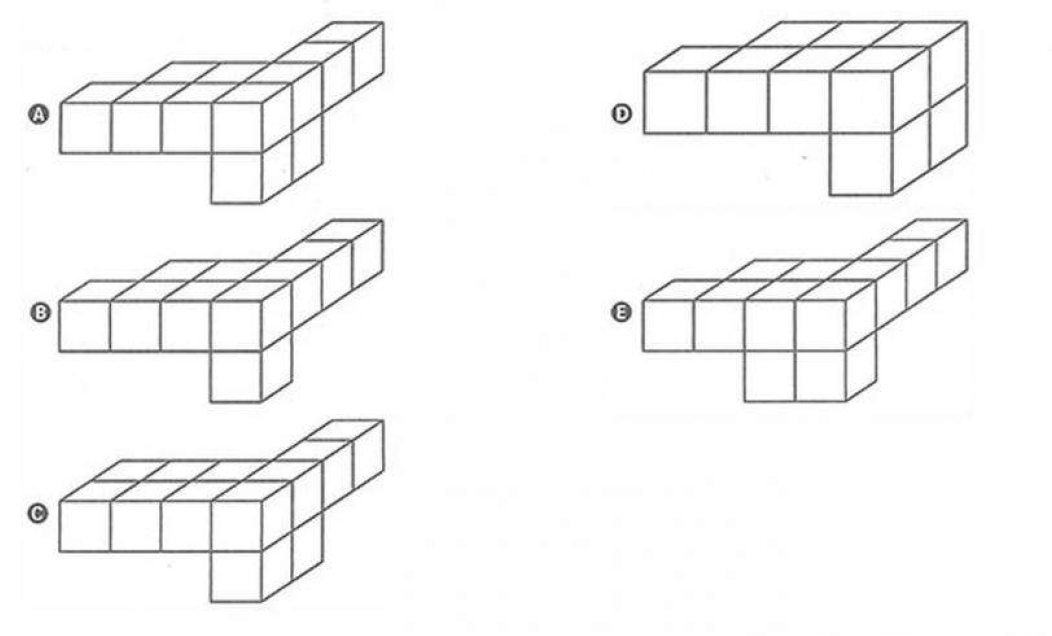
\includegraphics[width=8cm]{../figuras/q169(2)-2018.png}
\end{figure}

\begin{enumerate}
\item[a)]a
\item[b)]b
\item[c)]c
\item[d)]d
\item[e)]e
\end{enumerate}
